% 五号字体,开明式标点处理,不设置默认字体
\documentclass[UTF8,12pt,punct=kaiming,fontset=none]{article}
\usepackage[UTF8]{ctex}
\usepackage{fontspec}
\usepackage{float}
\usepackage{graphicx}
\usepackage{subcaption}
\usepackage{pgf-umlsd}
% 品红色链接和注释
% \usepackage[colorlinks=true, linkcolor=magenta, citecolor=magenta, urlcolor=magenta]{hyperref}
% 黑色链接和注释
\usepackage[colorlinks=true, linkcolor=black, citecolor=black, urlcolor=black]{hyperref}
\usepackage{geometry}
\usepackage{fancyhdr}
\usepackage{framed}
\usepackage{titlesec}
\usepackage{ragged2e}

\graphicspath{{figures/}}

% 字体
\IfFontExistsTF{Source Han Serif SC}
{
    \setCJKmainfont{Source Han Serif SC}
}
{
    % GitHub Actions
    \setCJKmainfont[
        Path=../fonts/ ,    
        Extension = .otf ,
        UprightFont = *-Regular ,
        BoldFont = *-Bold
    ]{SourceHanSerifSC}
}
\IfFontExistsTF{Source Han Sans SC}
{
    \setCJKsansfont{Source Han Sans SC}
}
{
    % GitHub Actions
    \setCJKsansfont[
        Path=../fonts/ ,    
        Extension = .otf ,
        UprightFont = *-Regular ,
        BoldFont = *-Bold
    ]{SourceHanSerifSC}
}
\IfFontExistsTF{DejaVu Sans}
{
    \setmainfont{DejaVu Sans}
    \setsansfont{DejaVu Sans}
}
{
    % GitHub Actions
    \setmainfont[
        Path=../fonts/ ,    
        Extension = .ttf ,
        BoldFont = *-Bold ,
        ItalicFont = *-Oblique ,
        BoldItalicFont = *-BoldOblique
    ]{DejaVuSans}
    \setsansfont[
        Path=../fonts/ ,    
        Extension = .ttf ,
        BoldFont = *-Bold ,
        ItalicFont = *-Oblique ,
        BoldItalicFont = *-BoldOblique
    ]{DejaVuSans}
}

% 布局
\geometry{a4paper,left=2cm,right=2cm,top=2.5cm,bottom=2.5cm}
\setlength{\headheight}{20pt}

% 页眉页脚
\pagenumbering{arabic}
\pagestyle{fancy}
\fancyhead[L]{· \hspace{0.1cm} \thepage \hspace{0.1cm} ·}
\fancyhead[C]{红\ 石\ 数\ 电\ 评\ 论\\\scriptsize{Review of Redstonic Digital Circuit}}
\fancyhead[R]{2022年1月(第1期)}
\fancyfoot[L,C,R]{}

% 标题
\title{\vspace{-1.5cm}基于石墙电路的随机存取存储器\vspace{-0.5cm}}
\author{@辰占鳌头,@NKID00\thanks{先进红石数电技术研讨组ARP}}
\date{}

% 参考文献标注
\newcommand*{\upcite}[1]{
    \textsuperscript{\cite{#1}}
}
\begin{document}
\maketitle
    \thispagestyle{fancy} % 首页页眉页脚
    \vspace{-0.7cm}

    % 摘要及关键词
    \begin{minipage}[c]{0.75\linewidth}
        \titleformat{\section}[wrap]{\sffamily\small\bfseries}{}{0cm}{}
        \titlespacing{\section}{2cm}{1ex}{0.4cm}

        \section{摘 \hspace{0.11cm} 要}
        \small Minecraft 1.16版本更新引入的石墙电路(墙电)提供了便捷的无延迟信号下传方案。
        结合经典的RAM方案,我们提出一种基于墙电的RAM方案。
        这一方案使用了竖式布线,可以纵向拓展到任意多位。同时,墙电的无延迟特性进一步降低了存取延迟,
        使得大位宽同步存取在16位及以上的CPU中成为可能。

    \end{minipage}
    \vspace{0.2cm}

    % 节标题格式
    \titleformat{\section}[hang]{\large\sffamily\bfseries}{\textmd{\thesection}}{0.5cm}{}
    \titlespacing{\section}{0cm}{0.5ex}{0.2ex}
    \setcounter{section}{-1}

\section{引言}
随机存取存储器(下称RAM)是指读写延迟与数据所在地址无关的存储器。
在Minecraft中存在一种体积较小的双片错位堆叠的RAM方案\upcite{ORE},见图\ref{fig:normalRAM}(a),每个比特占据$11\times 2\times 2$的堆叠体积。
因为控制读写的线路是竖半砖链,所以这种方案一般适用于竖式布线\upcite{Vertical}。
然而因为布线空间过小,为了避免存储数据与控制读写的半砖链串线,这个设计添加了额外的中继器,增加了延迟。
并且,单一半砖链仅能控制8位数据的读写,超过8位,读写控制线便需要利用双火把延长,从而引入2tick(下称t)的额外延迟,同时导致数据高位和低位的读写不再同步,见图\ref{fig:normalRAM}(b)。
而墙电作为无延迟的纵向导线弥补了这一缺陷。这里,我们利用了墙电体积小、不串线、无需续链的特点,提出了一个更快更紧凑的存储器。
这一方案有望运用在高位宽的(如32位)CPU中,或运用在其他需要快速随机存取的设备中。

如无特别说明,本文图例使用天蓝色混凝土/玻璃表示数据输入,黄绿色混凝土/玻璃表示数据输出,黄色混凝土/玻璃表示控制线路,见图\ref{fig:normalRAM}(a)。
\begin{figure}[t]
    \centering
    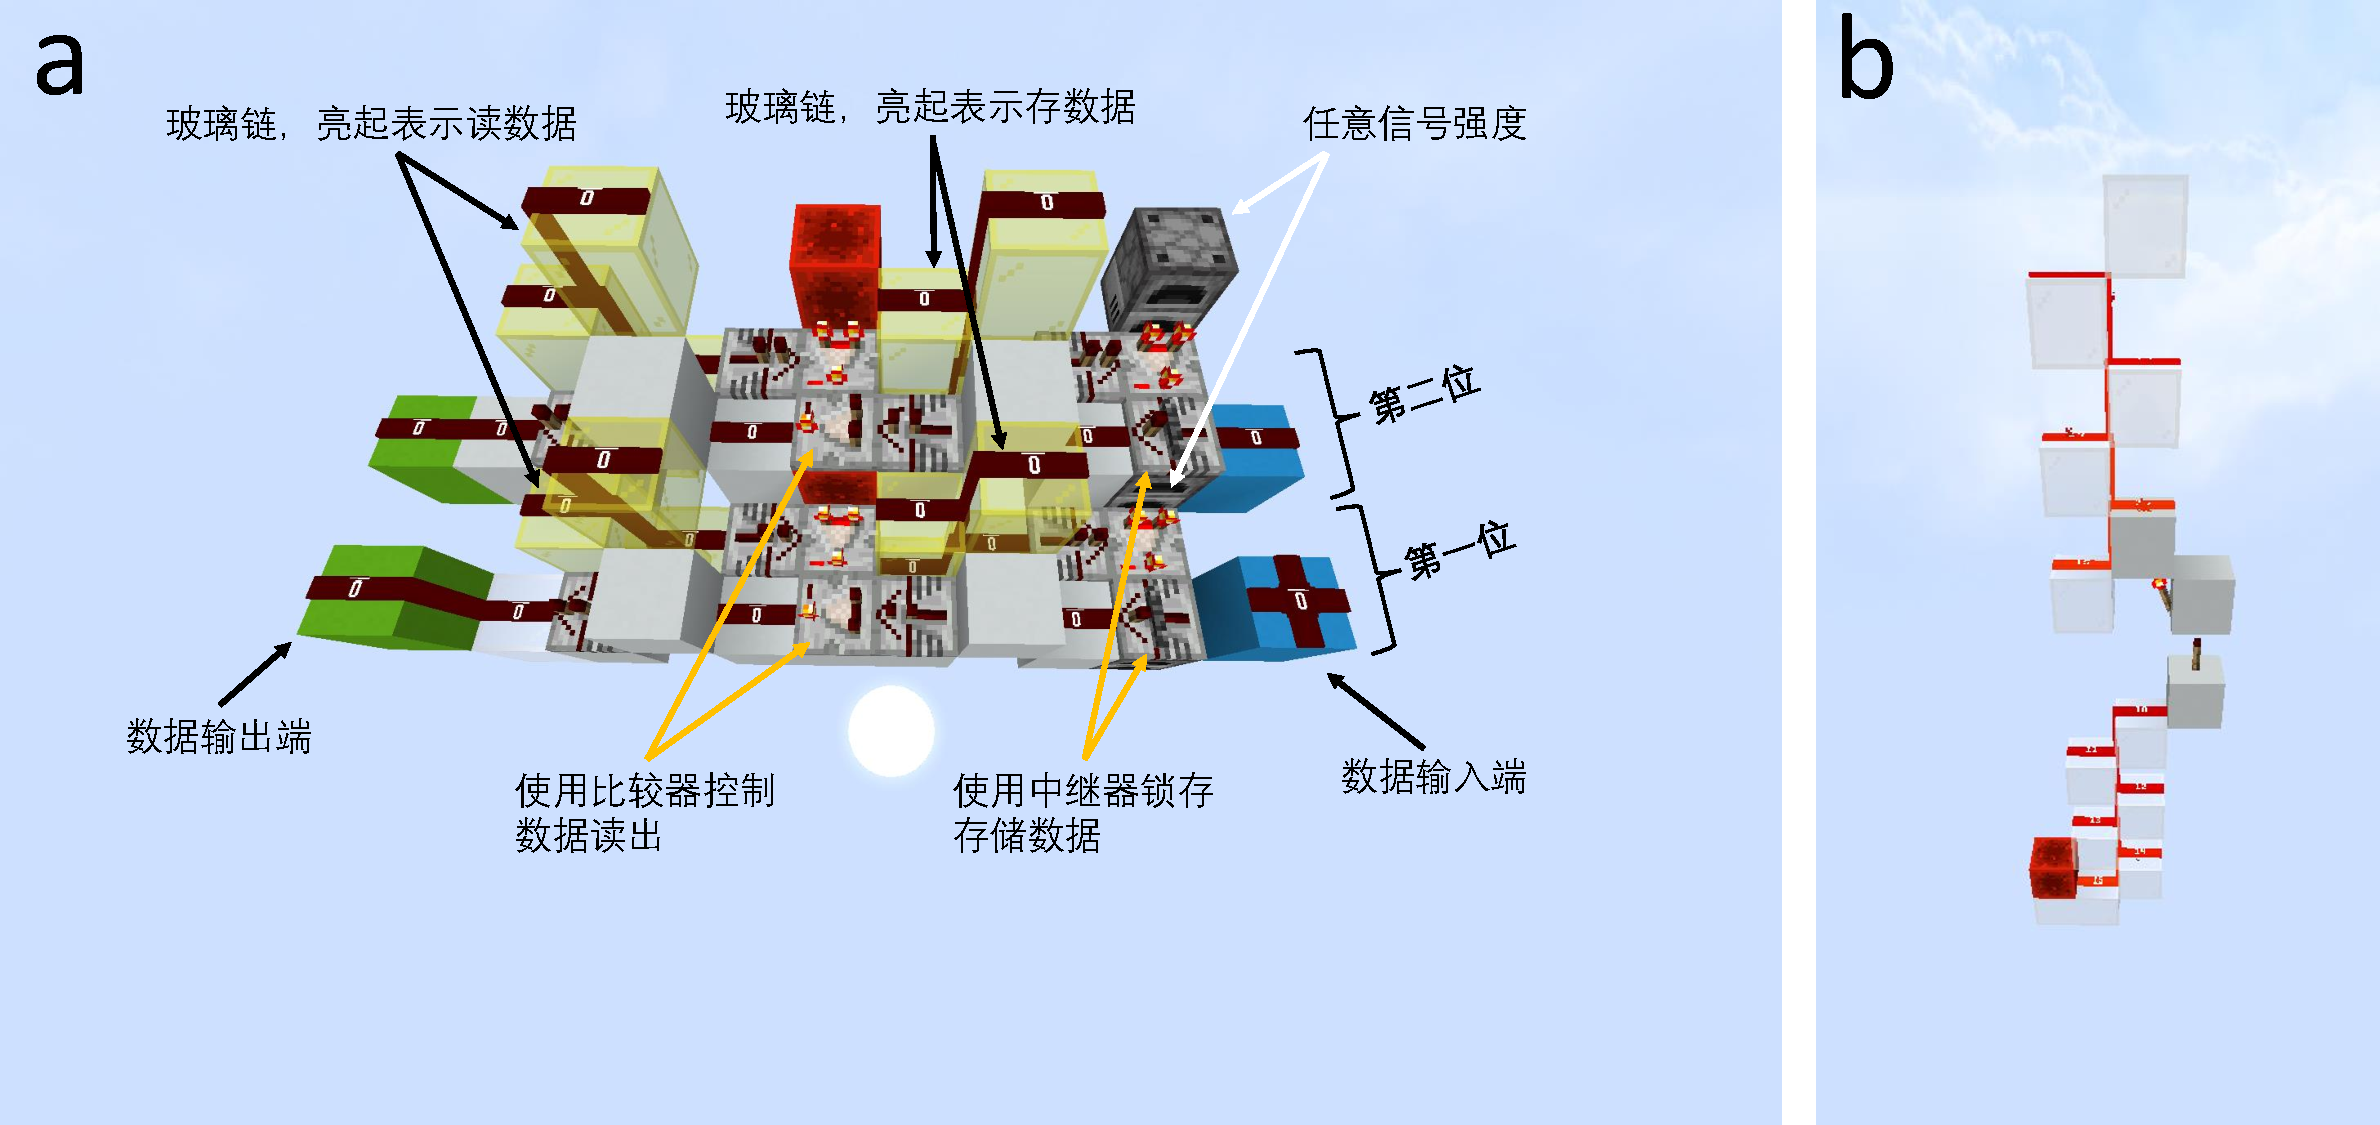
\includegraphics[width=.8\textwidth]{Fig1.pdf}
    \caption{(a) 使用半砖链的随机存储器原理图。可以以2格的层高向上堆叠。
    图中展示了横向双片错位堆叠,即第一位和第二位是紧密排布的,但高度上错开1格。
    这种错位堆叠是为了给比较器的信号源腾出位置。我们提出的墙电存储器也运用了错位堆叠。
    (b) 一种常规的半砖链续链方式,延迟为2t,同时会占用额外的空间。}
    \label{fig:normalRAM}
\end{figure}

\section{原理}
石墙(wall)会根据毗邻的方块改变连接形态,改变形态产生的方块更新可以被侦测器侦测\upcite{Wall}。
自1.16起,如图\ref{fig:wall}(a)一般的平石墙在侧面附着完整表面时,自被附着石墙往下的所有石墙会瞬间受到更新(这个更新是即时的, 无论处在哪个gametick阶段), 并立即转为柱垛,如图\ref{fig:wall}(b),
从而所有侦测这些石墙的侦测器都会侦测到石墙形态改变,并输出1t脉冲。
反过来,当方块被移除时,柱垛石墙会变平,侦测器会再次输出脉冲。
绝大多数方块都可以改变石墙形态,比如混凝土、玻璃、侦测器和其他石墙,而半砖、草径、中继器等则不会改变石墙形态。
有趣的是,竖起的活板门如果附着在石墙上,是可以改变石墙形态的,横放的活板门则不会。
活板门可以被红石控制,而且也是瞬间响应,所以一般使用活板门控制石墙电路。
需要注意的是,对于1t或2t时长的更新输入,侦测器只会输出一次脉冲,所以如果我们用1t或2t的脉冲去控制活板门,侦测器也只会输出1次脉冲。
不过,侦测器可以正常响应间隔1t的1t脉冲。也就是说,如果每2t就向活板门发送一个1t脉冲,石墙电路也能正常工作。

\begin{figure}[t]
    \centering
    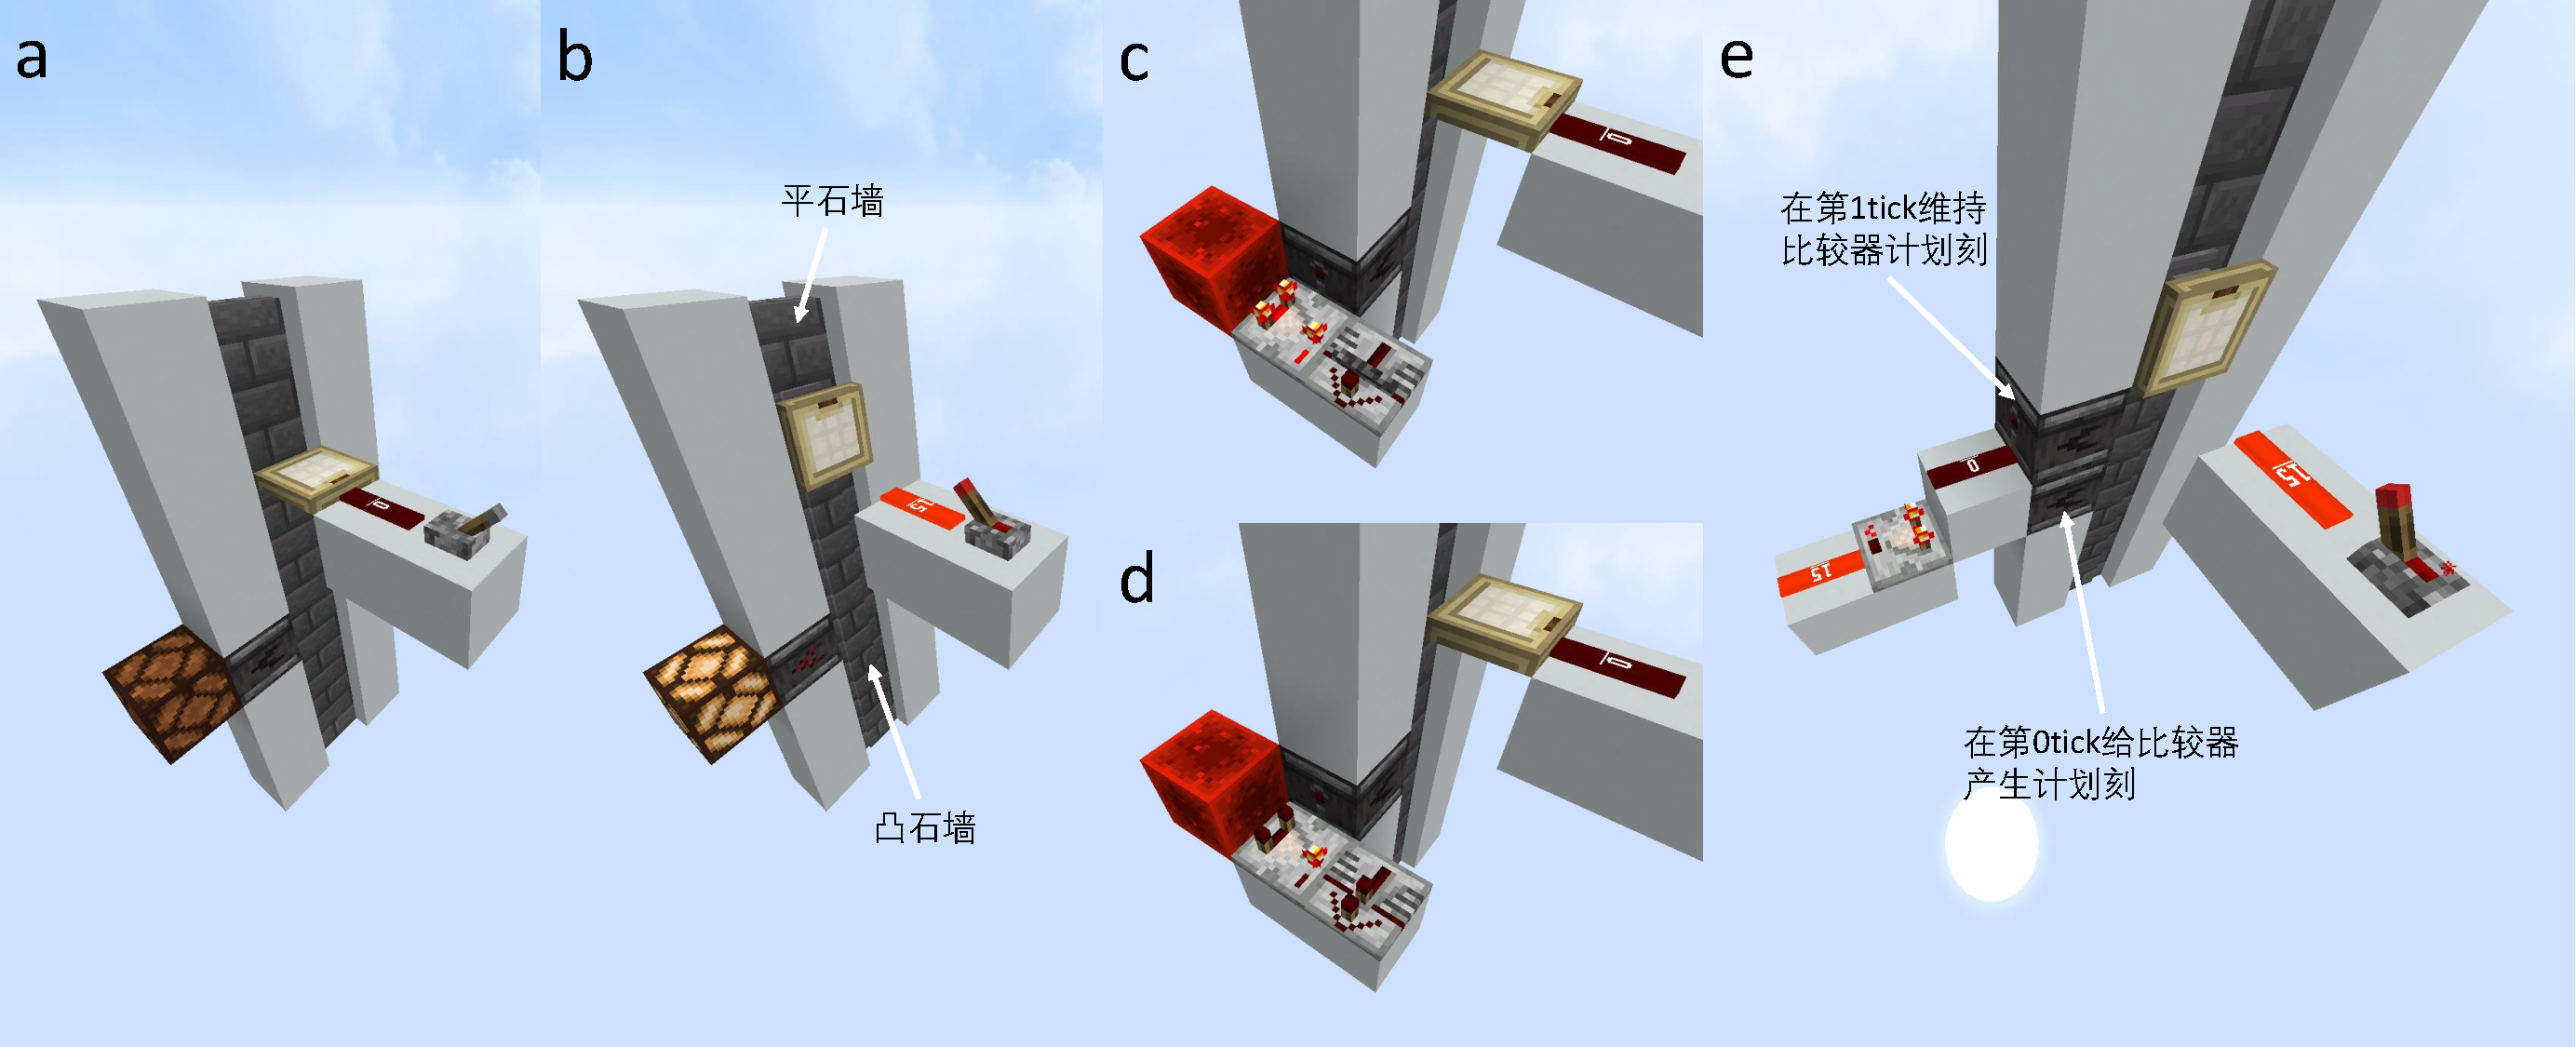
\includegraphics[width=.95\textwidth]{Fig2.pdf}
    \caption{(a) 平石墙,(b) 石墙顶端不变,自活板门往下石墙凸起,侦测器在活板门打开后1t进行响应并点亮了红石灯。
    (c) 利用比较器特性设计的锁存器,在侦测器侦测到石墙信号时锁存中继器。具体过程为:侦测器发出1t脉冲输入比较器侧面,比较器熄灭1t,而后亮起,完成对中继器的重新锁存。
    一般比较器只能响应2t及以上的脉冲,然而指向中继器的比较器例外,这一例外与计划刻有关。
    (d) 比较器被侦测器的1t脉冲屏蔽,中继器短暂解锁。
    (e) 另一个利用计划刻的设计。侦测器输出的1t脉冲可以借此通过比较器。}
    \label{fig:wall}
\end{figure}

在读写方面,我们利用了比较器的特性,设计出体积和延迟较小的存取结构。
与常规RAM相同,我们仍使用比较器锁存中继器的方式来存储数据。这一结构见图\ref{fig:wall}(c)(d)。
它利用了指向中继器的比较器可以响应1t脉冲的特性,这一特性源于计划刻优先级(tile tick)\upcite{TileTick}。
简单来说,Minecraft会为比较器的红石动作添加一个计划刻,并在下一tick按优先级和更新顺序执行。
如果在下一tick计划刻执行时,比较器后方或侧面的信号发生变化,不足以使比较器输出,那么比较器不会输出。这就是为什么一般比较器不能响应1t脉冲,只能响应2t及以上的脉冲。
然而指向中继器的比较器拥有较高的优先级,它的计划刻优先于输入信号改变,所以可以响应1t 。
对于图\ref{fig:wall}(e)的结构,上方的中继器可以在比较器计划刻执行时维持信号输入,所以这个比较器也可以响应1t脉冲。
尽管很有用,笔者不建议大量使用亚游戏刻设计(例如无延迟和计划刻),这些设计可能在一些情况下失效。

\section{设计}

将图\ref{fig:wall}(c)作为存储结构,图\ref{fig:wall}(e)作为读取结构,就是我们的墙电RAM方案,即图\ref{fig:wallRAM}(a)。其逻辑结构见图\ref{fig:wallRAM}(h)。
读取结构部分,我们通过添加红石火把(见图\ref{fig:wallRAM}(a)中的火把)来屏蔽比较器——存0时,屏蔽比较器,读取信号不能通过比较器;存1时不屏蔽,读取信号可以通过比较器。
%读取信号的逻辑可以认为是 $\mbox{\kaishu 存储值}\wedge \mbox{\kaishu 读取信号}$。
%比较器的逻辑为 $\mbox{\kaishu 后方}\wedge(\neg\mbox{\kaishu 侧面})$,而添加火把后,图\ref{fig:wallRAM}(a)中的读取逻辑变为 $\mbox{\kaishu 读取信号}\wedge(\neg(\neg\mbox{\kaishu 存储值}))=\mbox{\kaishu 读取信号}\wedge\mbox{\kaishu 存储值}$。
%这里,存储值指中继器锁存的信号,“读取信号”指侦测器发出的 1t 脉冲信号。
另一种类似的方案是使用所谓的“更新开关”,见图\ref{fig:wallRAM}(b)。
在存储1时,火把和铁轨熄灭,1号侦测器的信号可以通过铁轨传递给2号侦测器。
在存储0时,火把和铁轨亮起,1号侦测器充能铁轨时,铁轨不会产生更新,所以2号侦测器不会输出。
这样就完成了对输出的控制。

第一种方案,图\ref{fig:wallRAM}(a),每个比特占据$10\times 2\times 2$的体积,写入延迟为2t,读出延迟为2t,数据在存入后2t可用。
第二种方案,图\ref{fig:wallRAM}(b),每个比特占据$ 9\times 2\times 2$的体积,写入延迟为2t,读出延迟为2t,数据在存入后3t可用。
只要控制好时序,两种方案都可以接受数据以任意脉冲长度输入。而读出数据则是1t脉冲。
两种方案各有优劣。第一种方案中,数据可以被更快的使用,但是控制输出石墙信号必须在1t以上——图\ref{fig:wallRAM}(a)左侧的活板门不能接受1t脉冲,而第二种方案可以。
这可能降低读取频率。
当然,可以通过在比较器前加中继器来规避这一问题,然而这会引入额外的延迟。或者通过调制1t脉冲控制信号的计划刻来解决。这两个修改办法详见存档。
第二种方案在存储信号时会附带输出,因为图\ref{fig:wallRAM}(b)的2号侦测器会感知铁轨的变化,并且输出的信号并不是输入数据,而是输入的新数据与原数据的异或。
额外的输出可能干扰其他组件,也可能降低数据周转的频率。第一种方案则没有额外输出。

\begin{figure}[t]
    \centering
    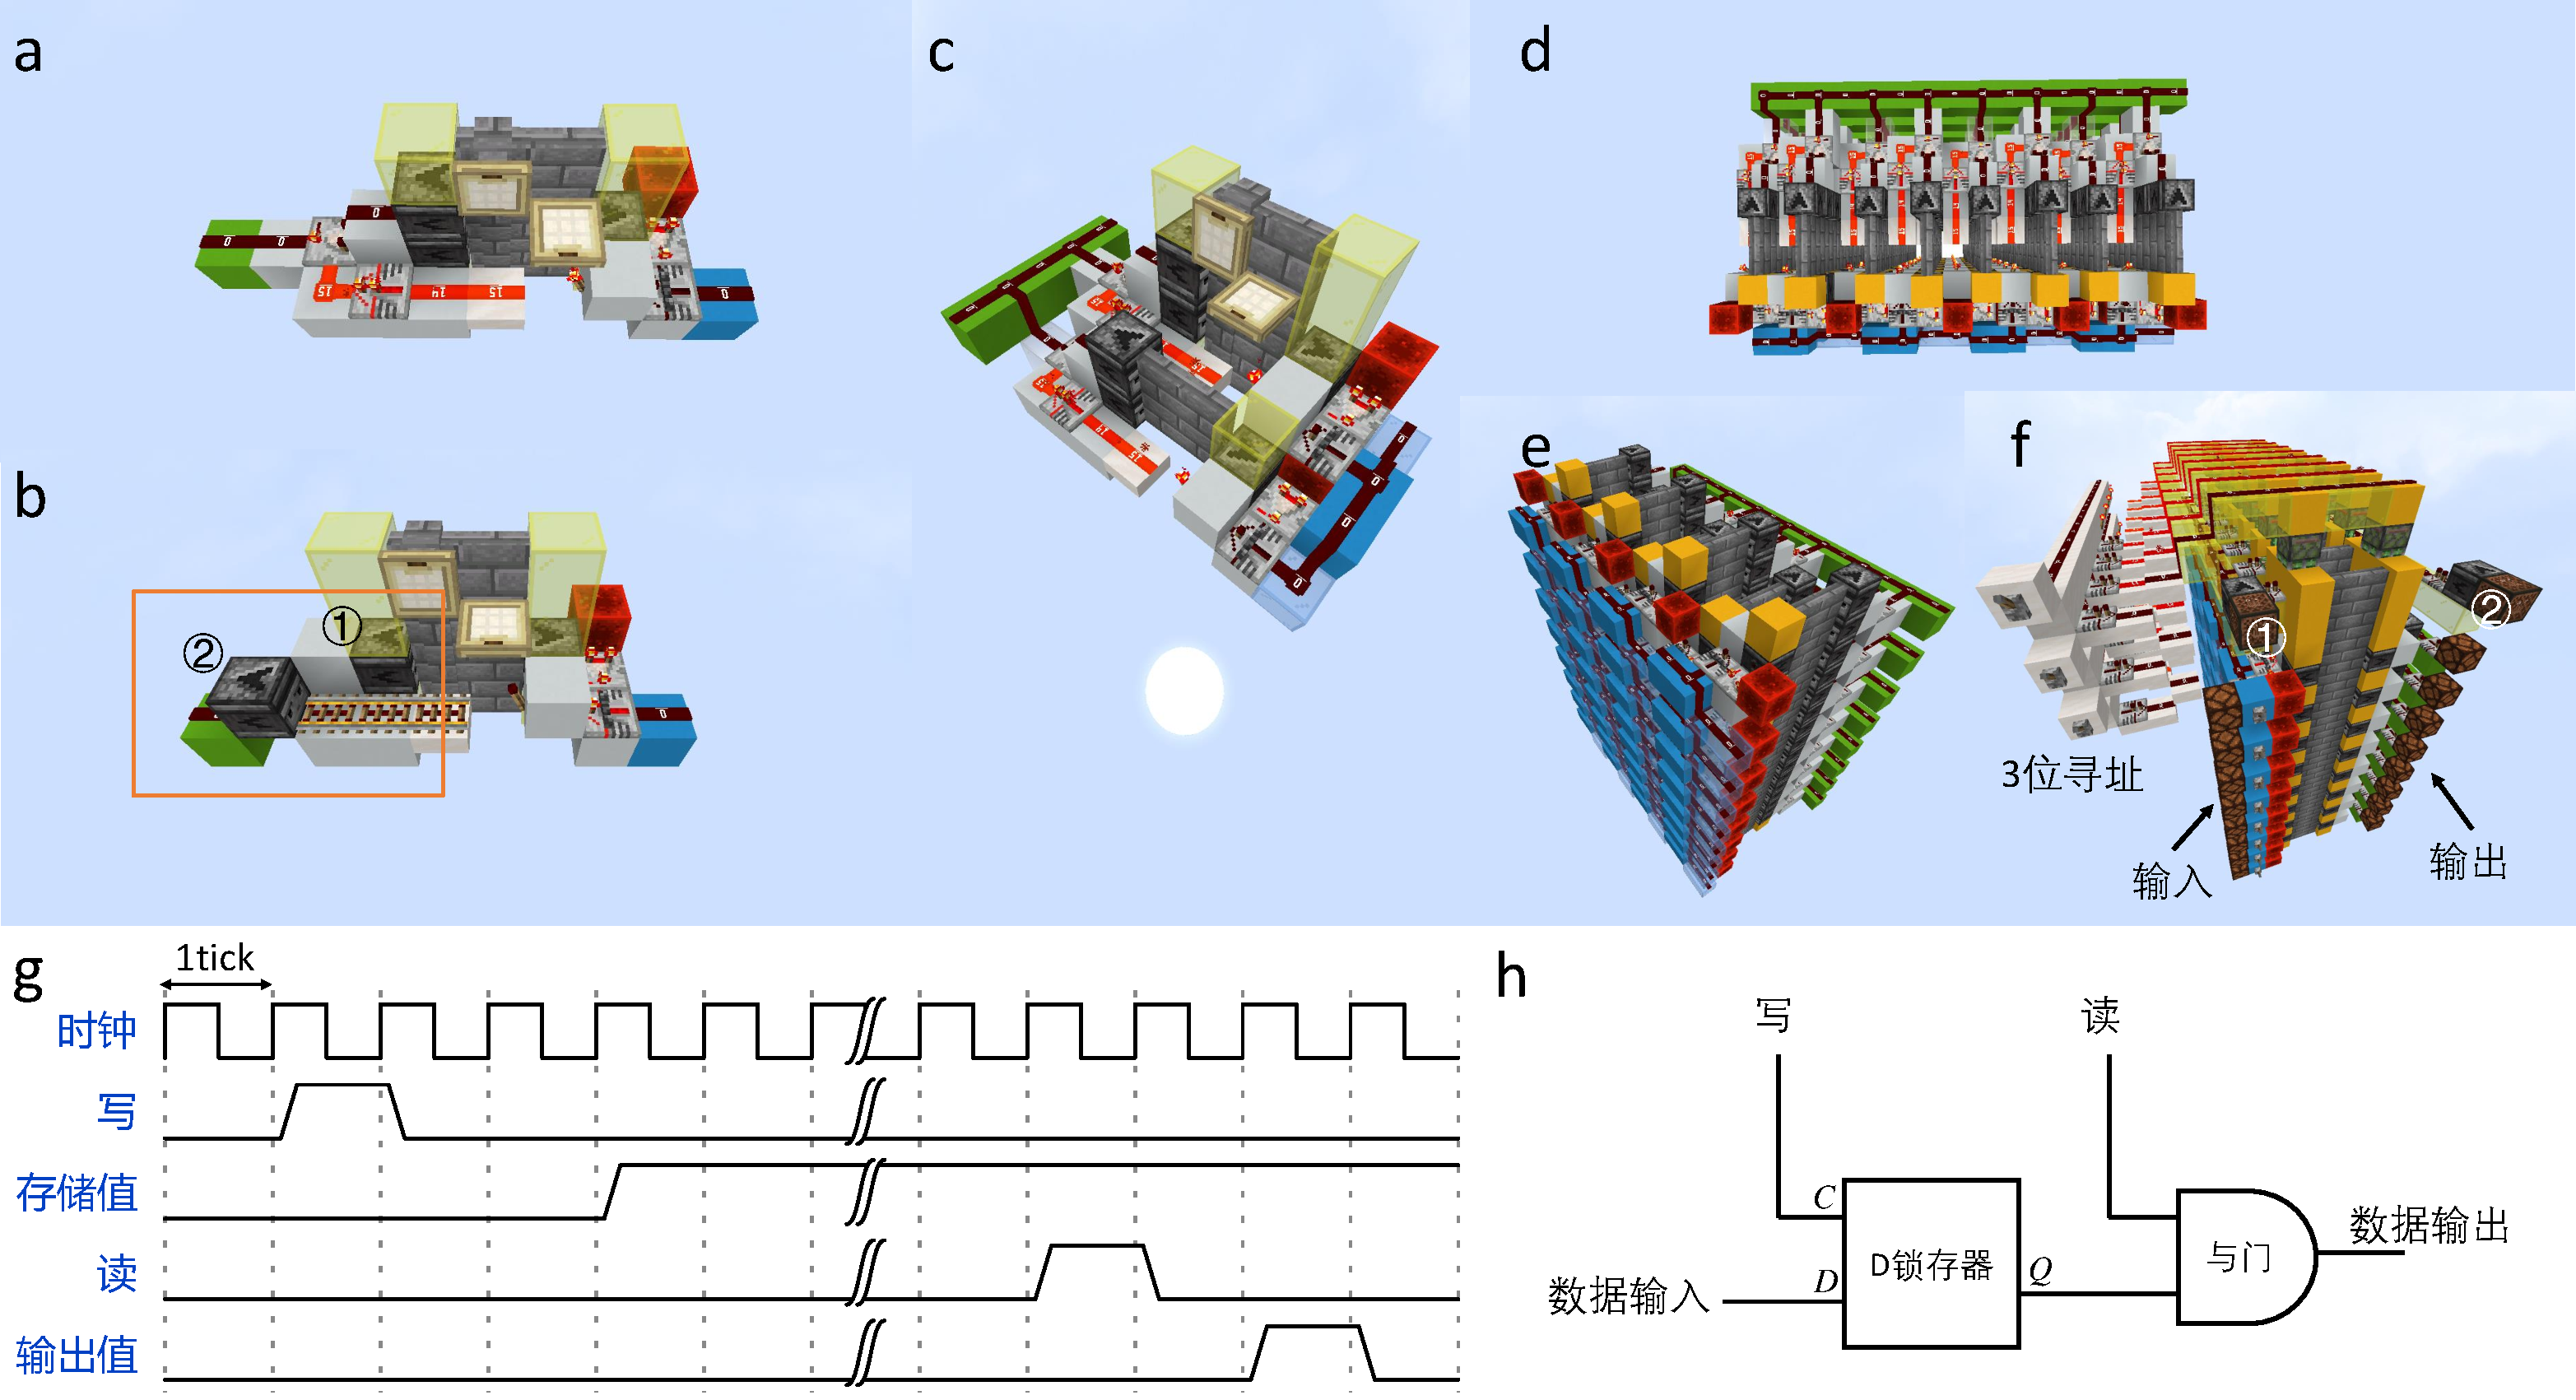
\includegraphics[width=.97\textwidth]{Fig3.pdf}
    \caption{(a) 使用比较器读取数据的墙电存储器方案,(b) 使用“更新开关”读取数据的墙电存储器方案。
    (c) 错位堆叠的方式,输入总线使用混凝土和玻璃交替,避免与相邻的比较器和红石块串线。(d) 堆叠后的8字节存储器俯视图。(e) 竖式数据输入总线的排布方式。
    (f) 寻址和输入输出控制。寻址采用竖式寻址,并配合活塞对控制线路进行通断。1号产生控制存储的脉冲,2号产生控制输出的脉冲。
    (g) 存储器时序图。(h) 存储器逻辑电路图。}
    \label{fig:wallRAM}
\end{figure}

包括修改方案在内的三种墙电方案都可以进行如图\ref{fig:wallRAM}(d)(e)的堆叠。
图中展示了8字节存储器的堆叠方案,适合竖式布线。由于墙电无需续链,故可以直接纵向堆叠以获得更高的位宽。
而进一步横向拓展则需要在输入输出总线和寻址线路上加中继器,每8个加1个中继器。这会带来额外的延迟,并需要详细计算时序。
不过在时序不敏感的电路里,这样的延迟是可以忽略不计的。
为了获得更小的体积,蓝色的输入总线使用玻璃和混凝土上下起伏,以避开比较器和红石块。
如果这种布线引发了额外的困难(比如强迫症),也可以将线路向外拓展一格,以期获得向输出总线一样平整的布线。
设计中用于给比较器提供信号强度的红石块也可以由其他容器替代。然而红石块卡顿更小,故在此仍推荐红石块。

不同于常规RAM,墙电RAM的控制线路位于存储器上端。在图\ref{fig:wallRAM}(f)中,我们展示了一个简单的控制方案。
我们使用常规的3位竖式寻址,控制8个字节的读写。指定地址对应的活塞会收起形成通路,其他地址对应的活塞仍然断路。
此时控制存储和输出的脉冲信号只能穿过通路,如此实现了对指定地址的读写控制。
从操作上来说,在输入数据后(拉下图\ref{fig:wallRAM}(f)输入端的拉杆),输入指定地址(拉下图\ref{fig:wallRAM}(f)寻址端的拉杆),然后右击1号音符盒产生一个脉冲,存储当前输入的数据到指定地址。
变更地址和输入,数据不会消失,除非重新写入。读出数据同样要先输入指定地址(拉下图\ref{fig:wallRAM}(f)寻址端的拉杆),而后右击2号音符盒产生一个脉冲,数据将以1t脉冲形式从输出端输出。
注意,第一种方案(图\ref{fig:wallRAM}(a)所示),控制输出的脉冲是2t,而对于第二种方案和修改方案是1t。
在示例存档中,我们通过改变2号音符盒后的中继器延迟来实现这一点。

\section{总结}
墙电随机存储器在体积和速度方面均由于传统的基于半砖链的随机存储器。
其无需续链的特点为高位宽同步数据处理带来便利。我们甚至有望实现全部基于墙电的“下端序”竖式布线CPU。这种CPU有可能拥有更好的性能。
而墙电存储器小巧快速的特点,也让它能在大型红石生电领域有所运用。

\bibliographystyle{unsrt}
\bibliography{reference.bib}

\end{document}